\documentclass{article}
\usepackage{graphicx}
\usepackage{listings}
\usepackage{siunitx}
\usepackage{placeins} %chatGPT suggestion to prevent figures getting rendered weirdly

\setlength{\topmargin}{-2cm} 
\setlength{\textheight}{650pt}
\begin{document}

\section*{Implementation}
In this project I attempted to model the linear Advection-Diffusion equation by Implementing 4 finite difference schemes. 
the coding for this project was going very smoothly until I had to implement output.f90, advec\_diff.f90 and plotter.py.
I believe that most of my finite difference scheme implimentations are correct and if I had started earlier and given myself 
more time I would have been able to flesh out the output portion of the code better. 

\section*{Questions}
\subsection*{a}
I was unable to figure out how to implement a way to only write the times when t/tmax = 0, 0.2, 0.5, 0.8, 0.1 I was able to write out the solution at every time step, 
but then when I pivoted to work on my solution to the advection portion, this part of the code broke and I didnt have time to look back to find out what's wrong.
\subsection*{b}
at grid size N = 32, our solition reaches stability at tmax = 1.9184891327856113, at grid size N = 128, our solution reaches stability at tmax = 1.8369945275333388, however our run time is much longer
this shows tells us that our grid size helps us determine when our solution will reach stability which can effect tmax
\subsection*{c}
when tdiff fails to satisy the CFL condition our solution is unstable and we arent garunteed to ever reach stability
\subsection*{d}
at grid size N = 32 and k = 1.156, our solition reaches stability at tmax = 1.9184891327856113. when we keep the grid size the same but increase k by a factor of 10 to 
k = 11.56 our solution reaches stability at tmax = 0.21326401654410712 which is much much faster, this is because our k value represents diffusivity which you can see from the 
units $cm^3/s$ is a measurement of the rate that heat diffuses over a cubic centimeter, by increasing it we diffuse faster, and by decreasing it we diffuse slower
which in turn causes us to reach stability earlier or later.
\subsection*{e}
not super sure how to do this

\newpage

\subsection*{f}
    these plots are using grid size n = 64, and a = 1, my code can produce other grid sizes but i did not have time to do this
    \begin{figure}[htbp]
        \centering
        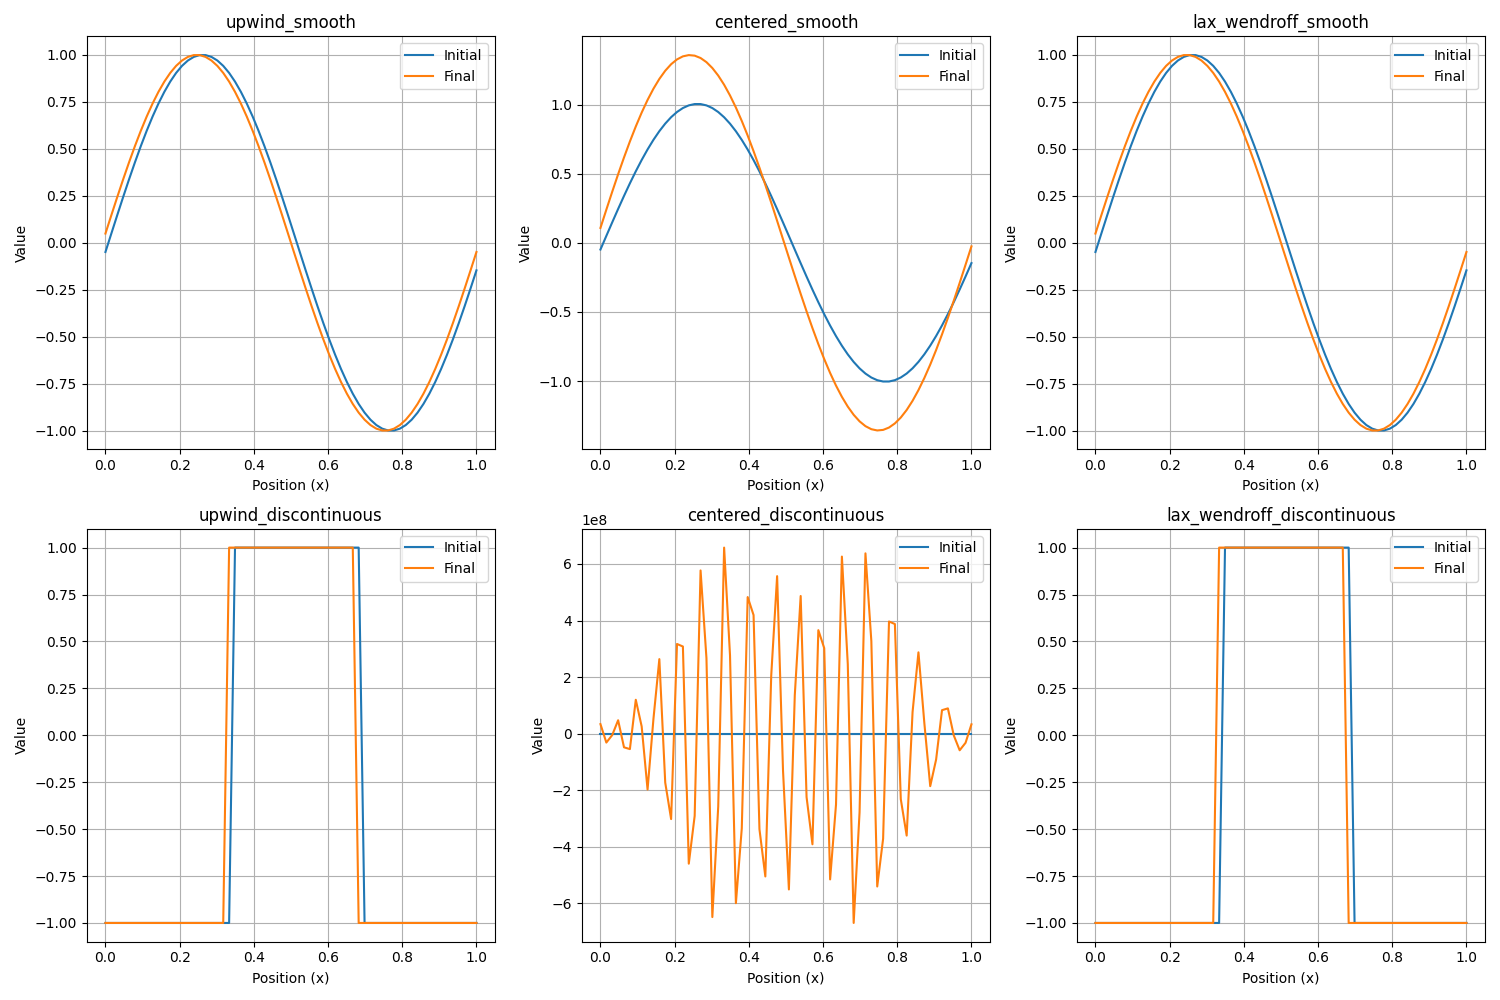
\includegraphics[width=0.8\textwidth]{../code/figures/advection_comparison.png}
        \caption{comparison between discrete and continuous advection schemes}
        \label{fig: solutions.png}
    \end{figure}

    \FloatBarrier
    it appears that the centered scheme is the least accurate over both continuous and discrete initial conidtions, it seems like there is minimal difference
    between the upwind and lax-wendroff schemes. 

\subsection*{g}
I did not have time to try g

\section*{conclusion}
this was a very fun project and I should have started much sooner, I let it lull me into a false sense of security because everything up until the plotting seemed like smooth sailing
I believe that all my code is operational and I would only need another day to fix the issues that I currently have. 

\end{document}
